\documentclass{article}

\usepackage{geometry}
\usepackage{makecell}
\usepackage{array}
\usepackage{multicol}
\usepackage{setspace}
\usepackage{changepage}
\usepackage{booktabs}
\usepackage{graphicx}
\usepackage{cprotect}
\usepackage{float}
\newcolumntype{?}{!{\vrule width 1pt}}
\newcommand{\paragraphlb}[1]{\paragraph{#1}\mbox{}\\}
\renewcommand\theadalign{tl}
\setstretch{1.10}
\setlength{\parindent}{0pt}

\geometry{top=12mm, left=1cm, right=2cm}
\title{\vspace{-1cm}Netzwerktechnologien Übung 7}
\author{Andreas Hofer}

\begin{document}
	\maketitle
	\section{Netzwerksetup}
	Ich musste ein paar der früheren Bilder erneut aufnehmen, weshalb einige Konfigurationen aus späteren Nummern bereits vorhanden sind, was jedoch hoffentlich kein Problem ist.
	\subsection{Laptop}
	\begin{figure}[H]
	\centering
	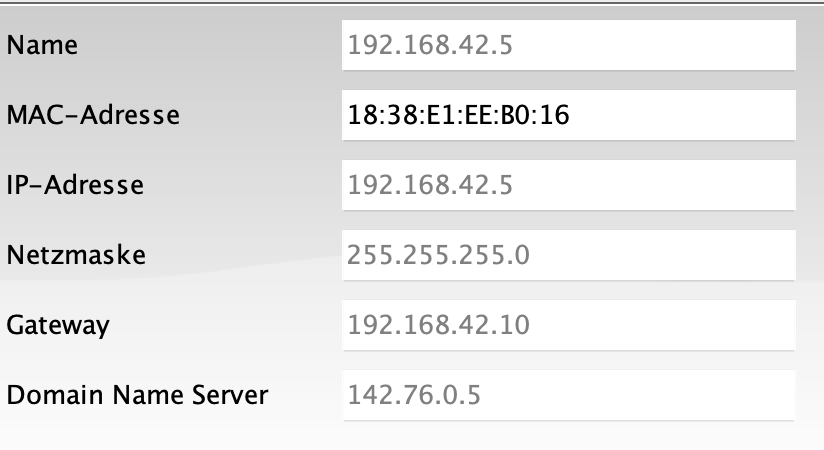
\includegraphics[scale=0.5]{1.1.png}
	\caption{Laptoptkonfiguration mit DHCP}
	\end{figure}
	\subsection{Ausführung}
	\begin{figure}[H]
	\centering
	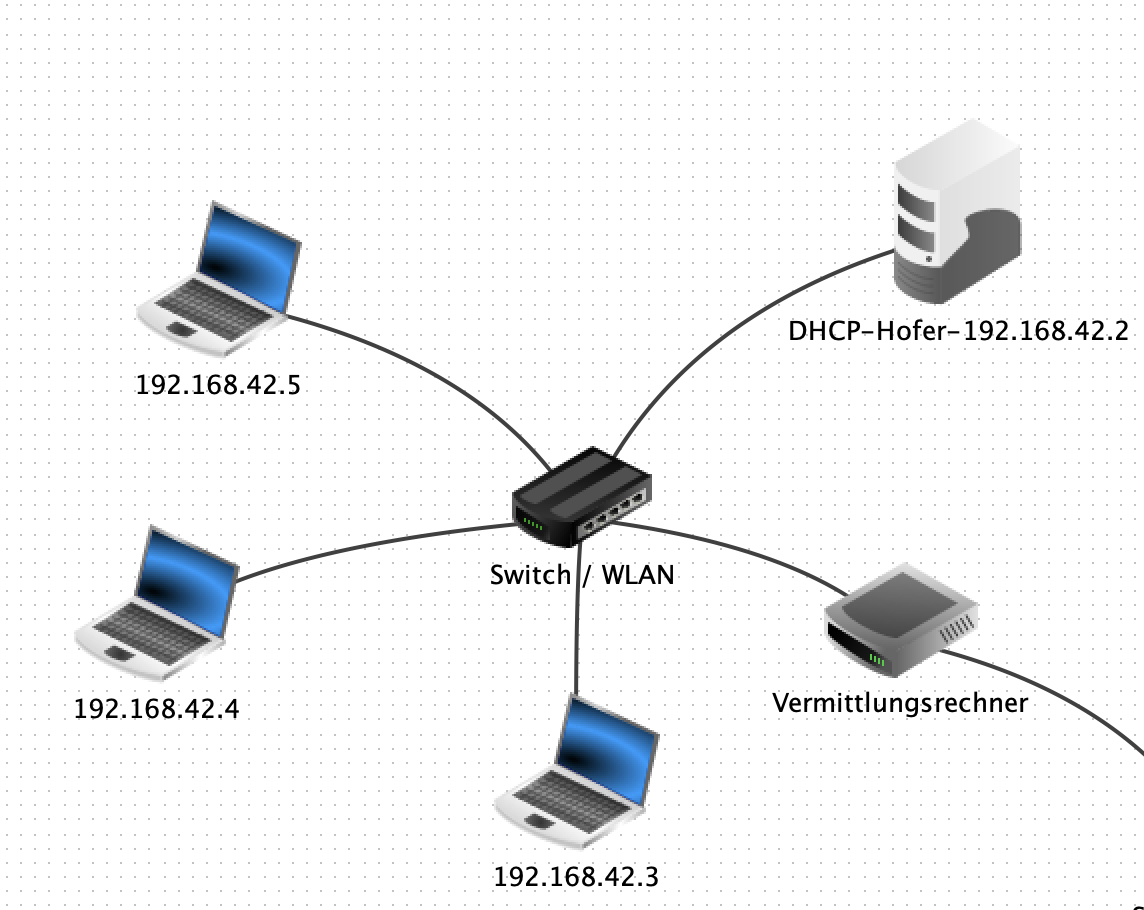
\includegraphics[scale=0.5]{1.2.png}
	\caption{IP Vergabe im Netzwerk}
	\end{figure}
	\subsection{DHCP Server}
	\begin{figure}[H]
	\centering
	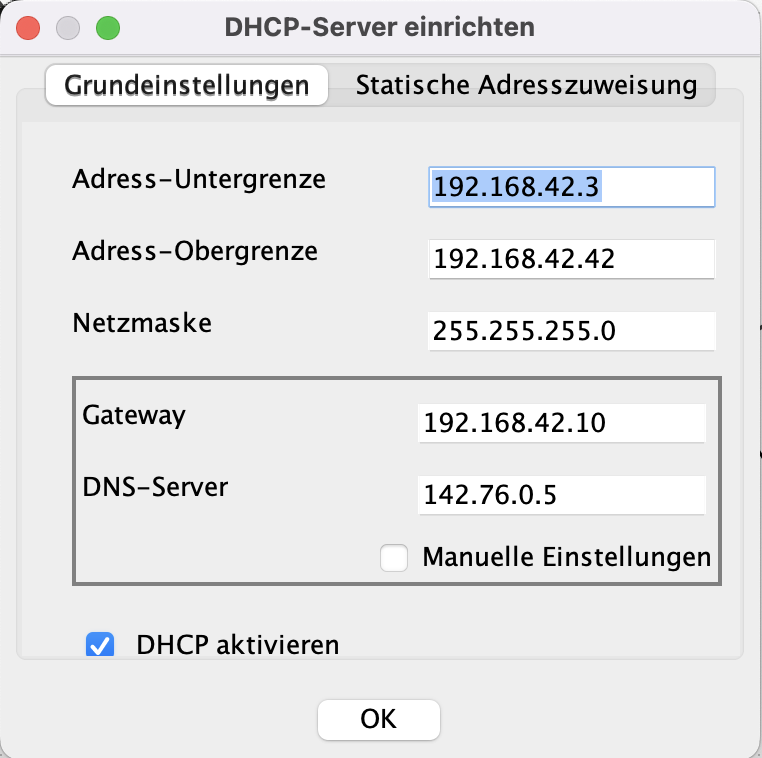
\includegraphics[scale=0.5]{1.3.png}
	\caption{DHCP Konfiguration}
	\end{figure}
	\section{Gateway}
	\subsection{Netzwerkaufbau}
	\begin{figure}[H]
	\centering
	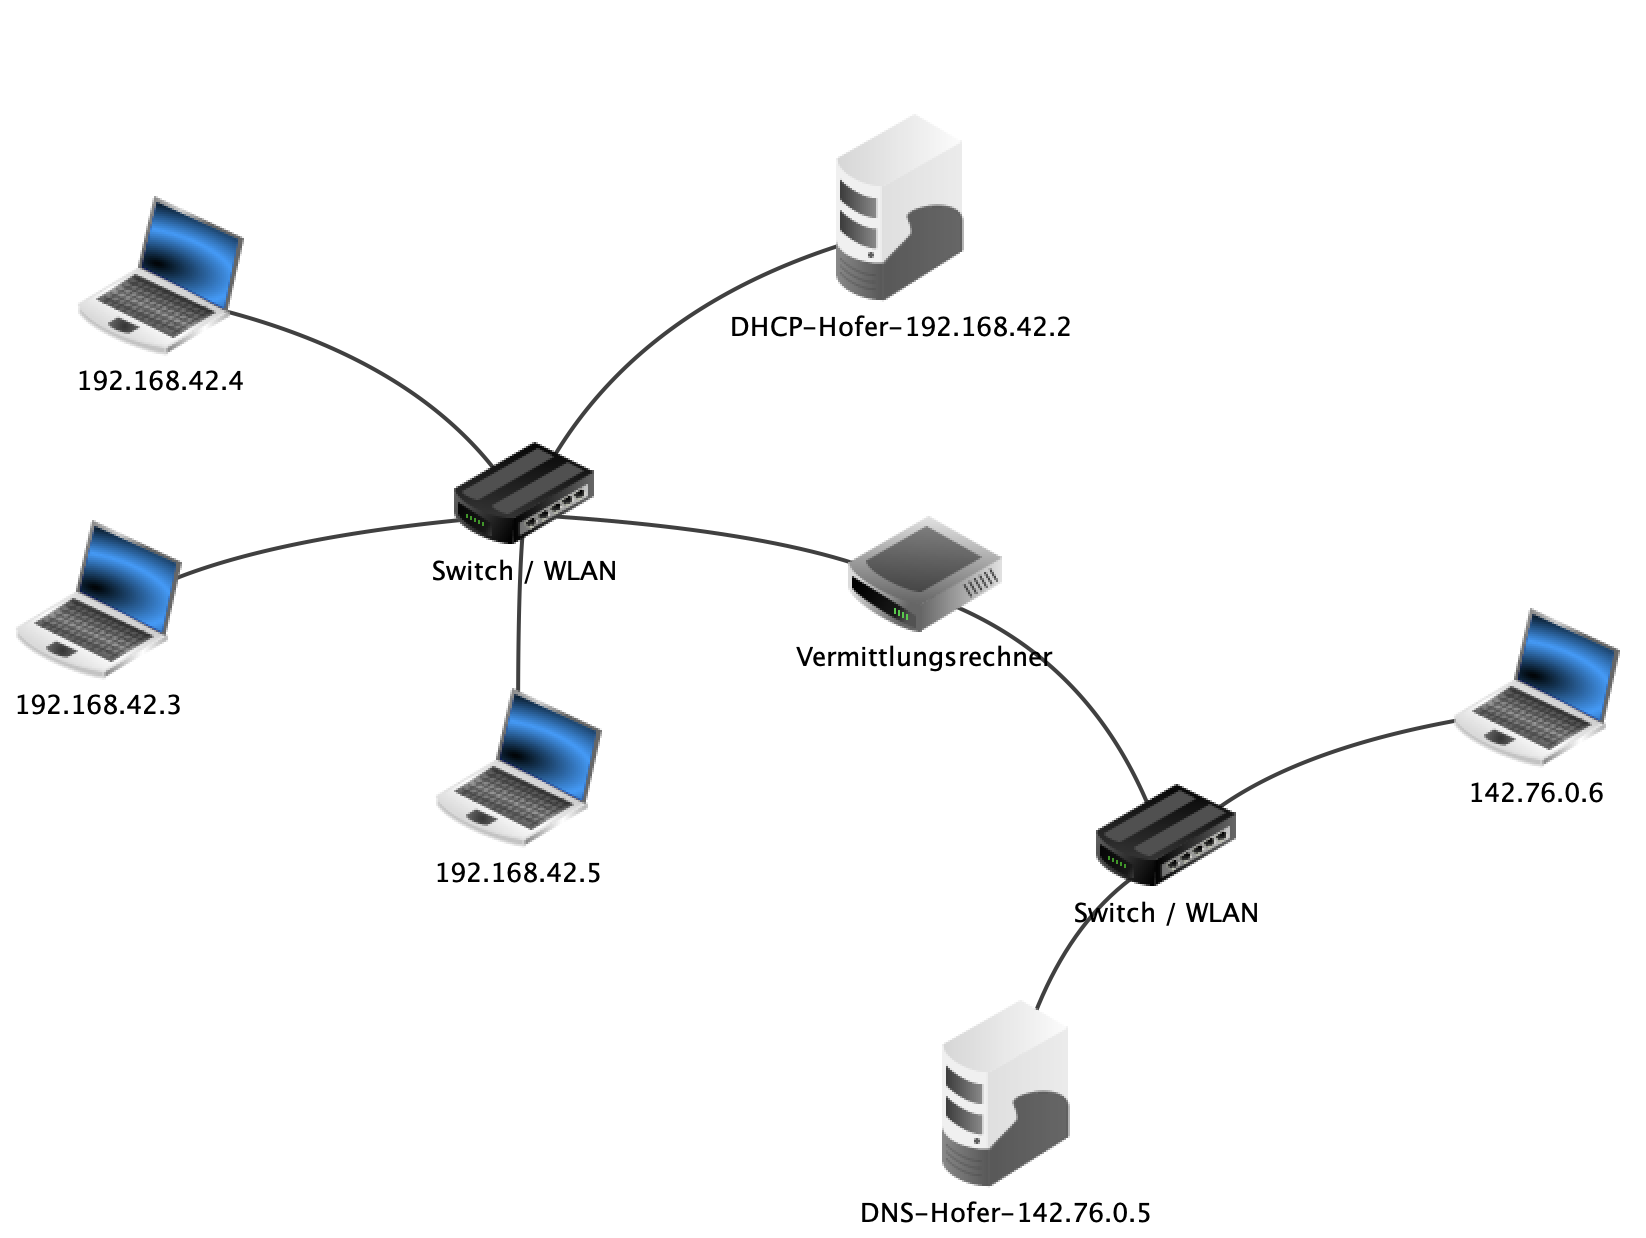
\includegraphics[scale=0.4]{3.1.png}
	\caption{Ausgeführtes Netzwerk}
	\end{figure}
	\subsection{DHCP Konfiguration}
	\begin{figure}[H]
	\centering
	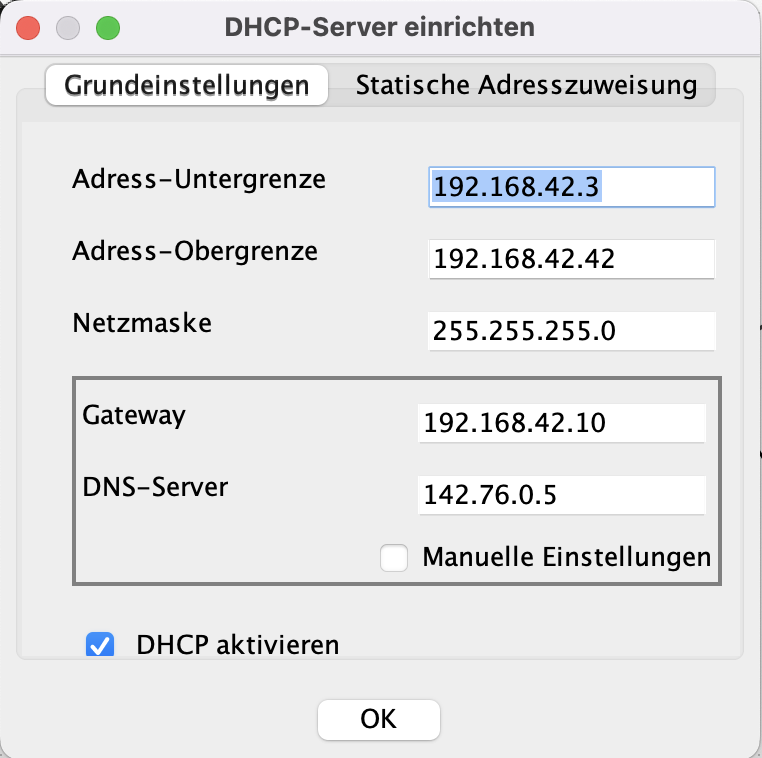
\includegraphics[scale=0.5]{1.3.png}
	\caption{DHCP Konfiguration mit Standard Gateway und DNS Server}
	\end{figure}
	\subsection{Vermittlungsrechner}
	\begin{figure}[H]
	\centering
	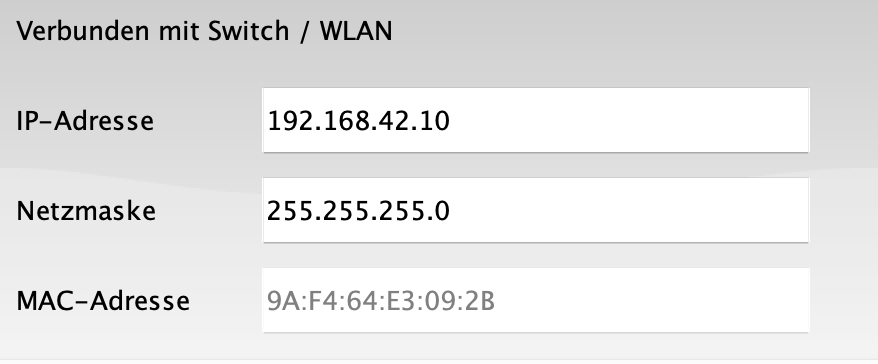
\includegraphics[scale=0.4]{2.31.png}
	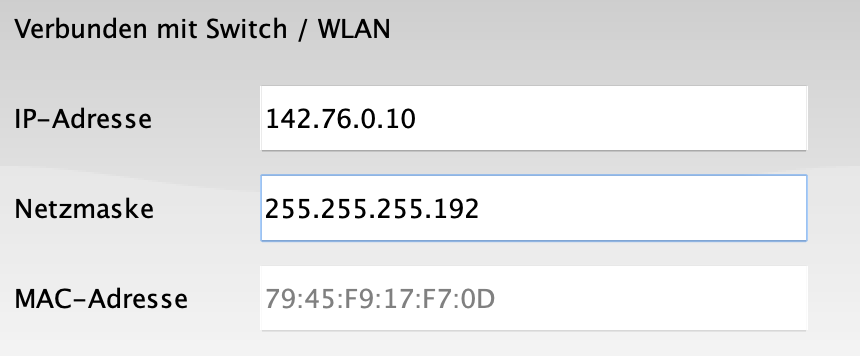
\includegraphics[scale=0.4]{2.32.png}
	\caption{Einstellung des Vermittlungsrechners}
	\end{figure}
	\subsection{Ping}
	\begin{figure}[H]
	\centering
	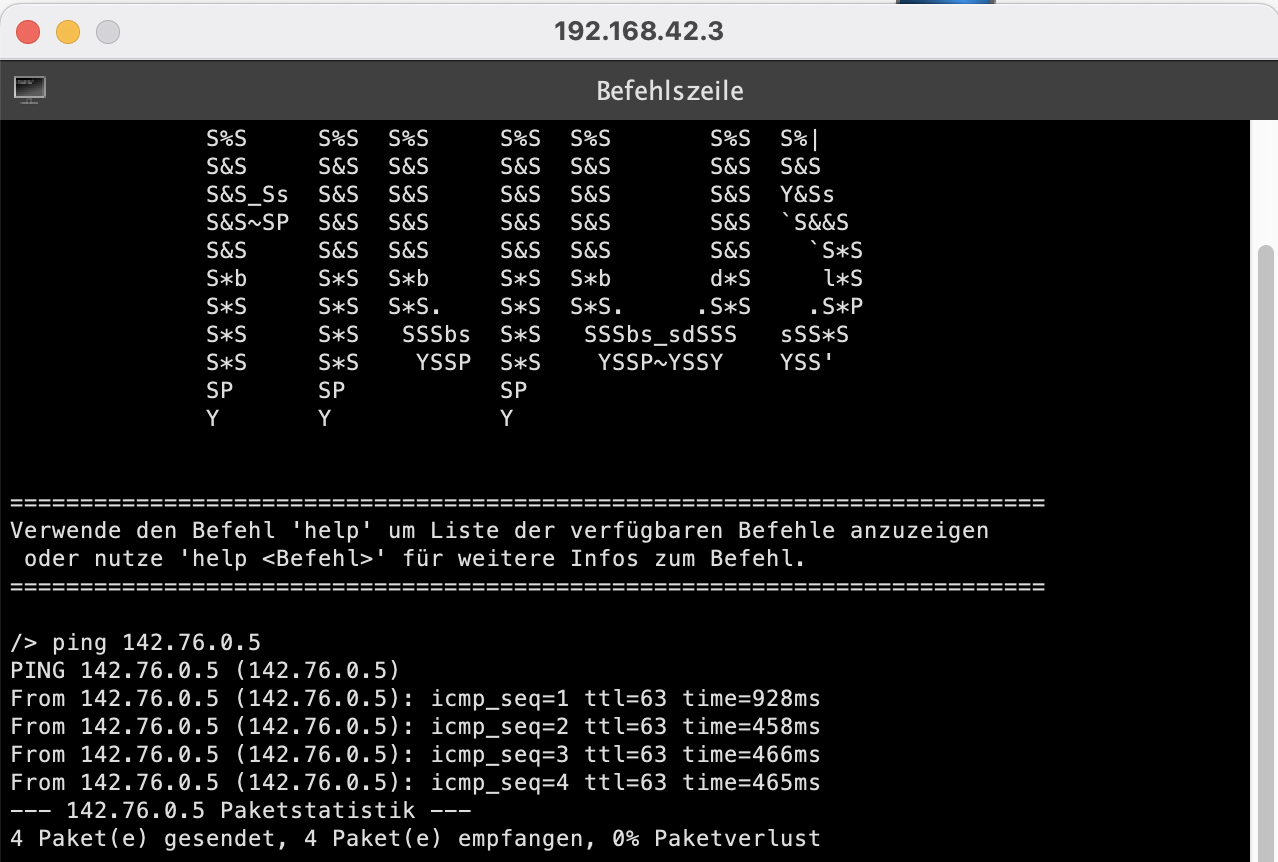
\includegraphics[scale=0.4]{2.4.png}
	\caption{Ping an den DNS Server}
	\end{figure}
	\section{DNS Server}
	\subsection{Netzwerkaufbau}
	\begin{figure}[H]
	\centering
	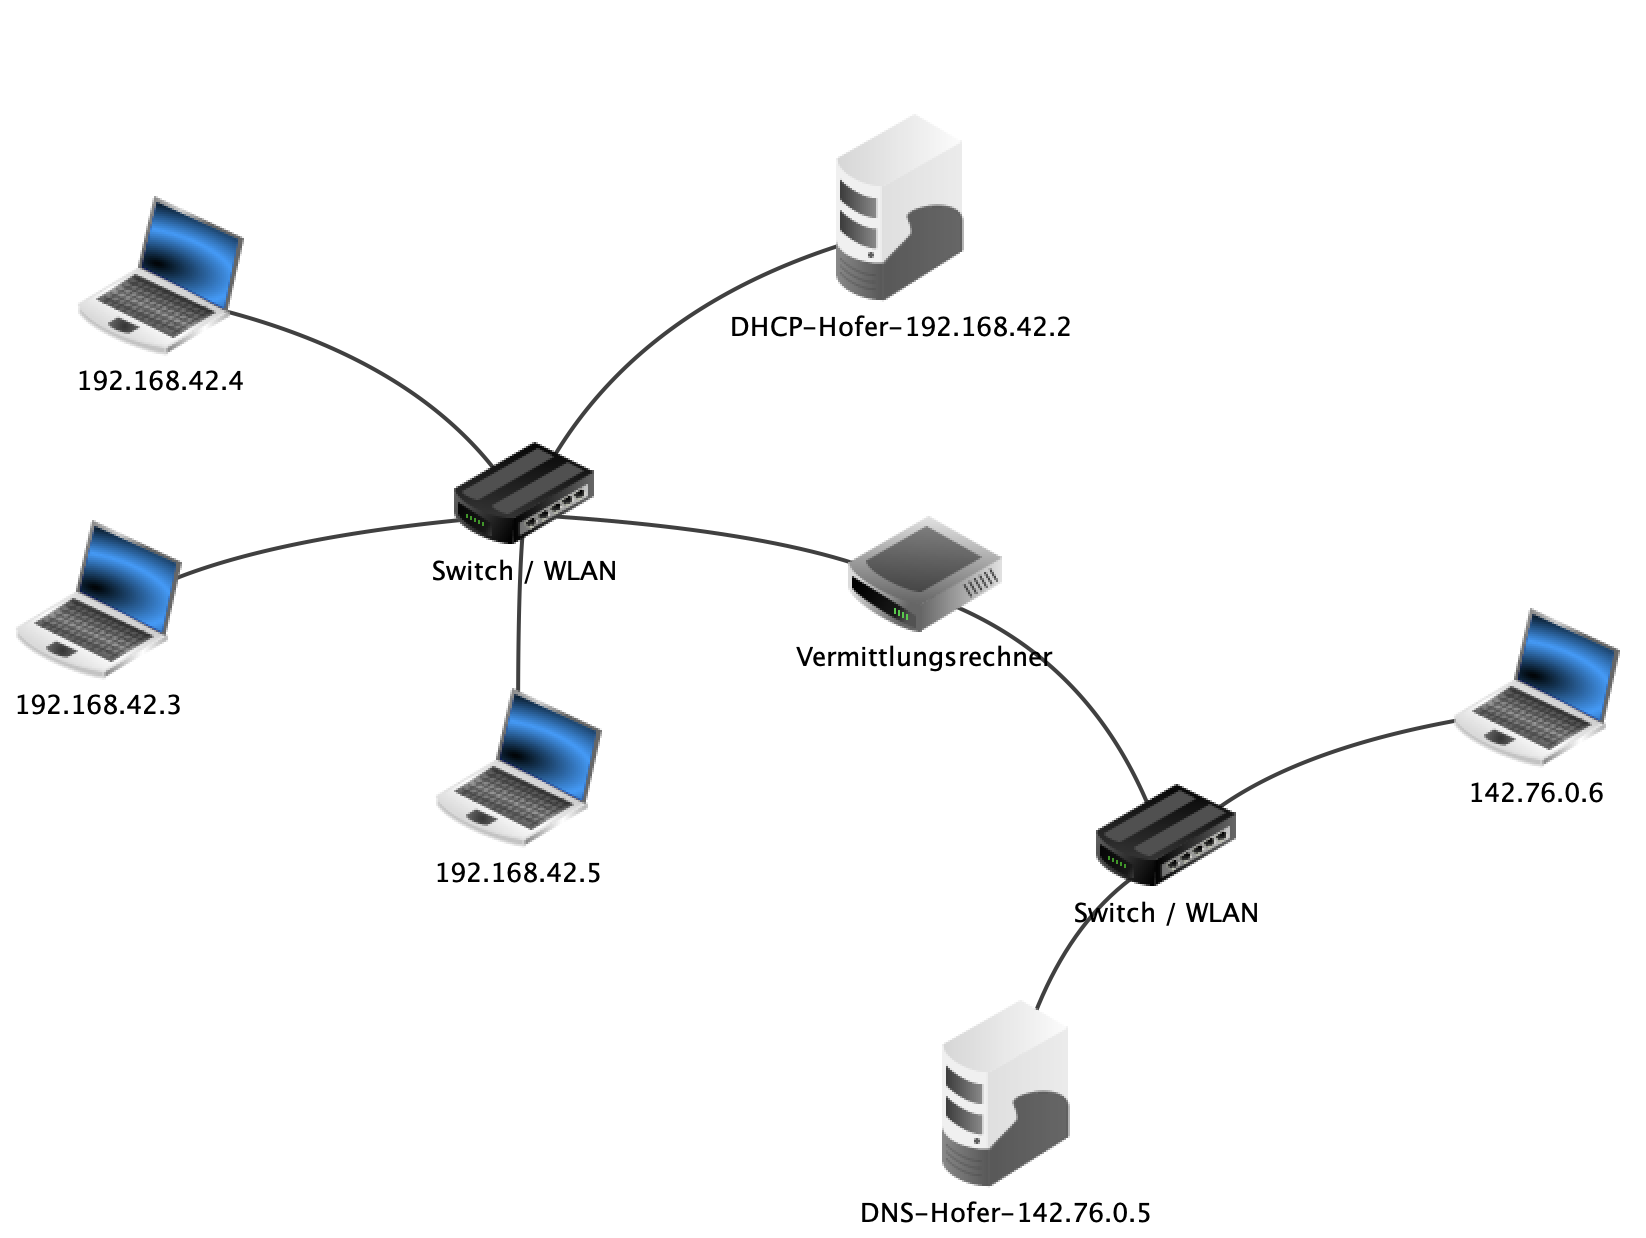
\includegraphics[scale=0.4]{3.1.png}
	\caption{Netzwerkaufbau mit Webserver}
	\end{figure}
	\subsection{DNS Server}
	\begin{figure}[H]
	\centering
	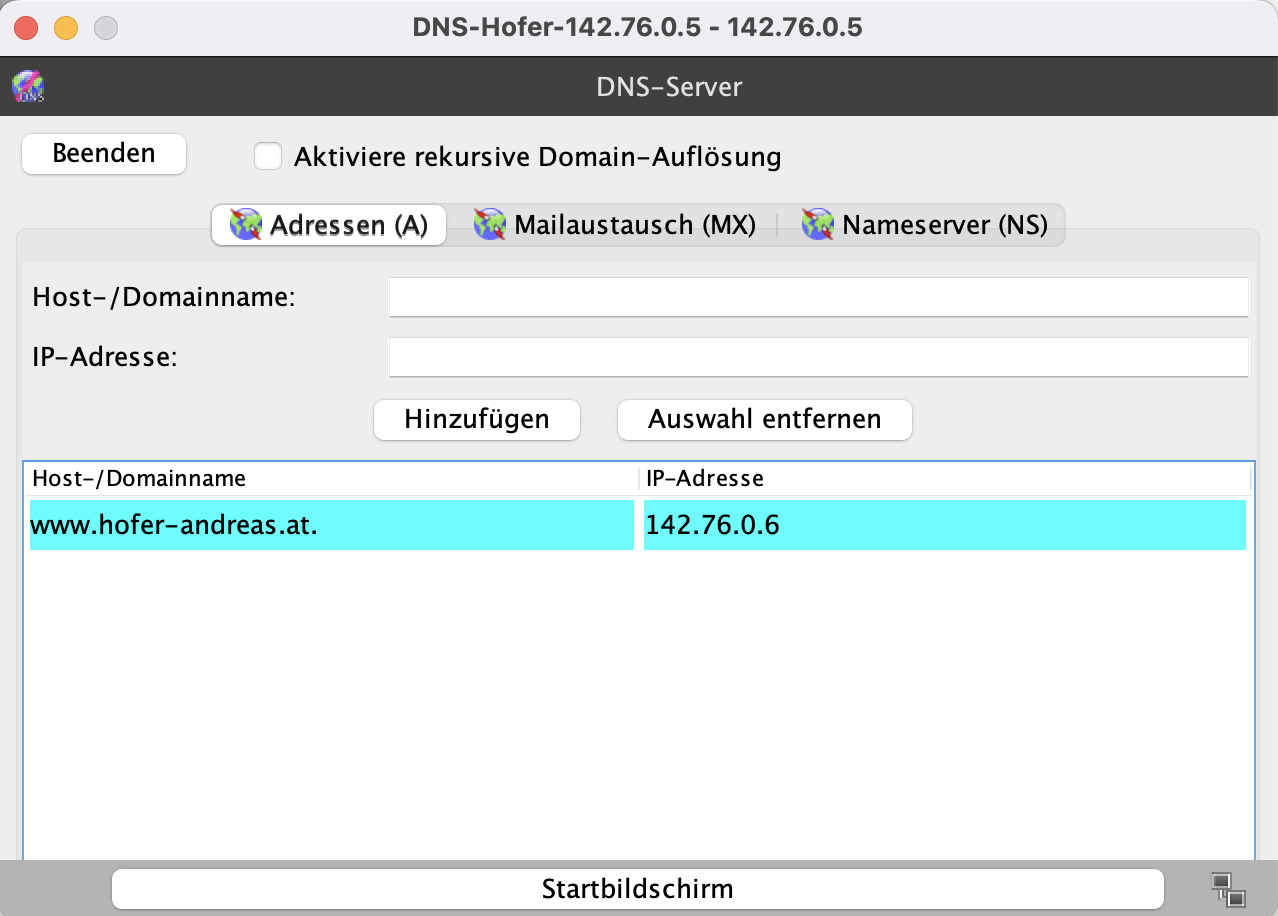
\includegraphics[scale=0.5]{3.2.png}
	\caption{DNS Server mit Webserverkonfiguration}
	\end{figure}
	\subsection{Webserver}
	\begin{figure}[H]
	\centering
	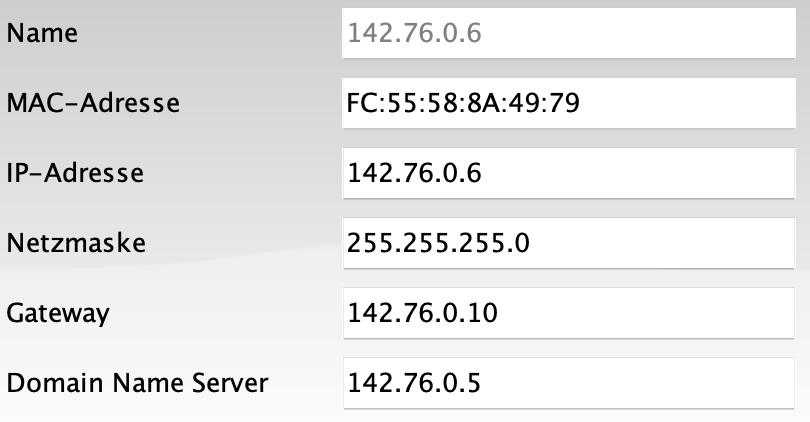
\includegraphics[scale=0.5]{3.3.png}
	\caption{Konfiguration des Webservers}
	\end{figure}
	\subsection{Vermittlungsrechner}
	\begin{figure}[H]
	\centering
	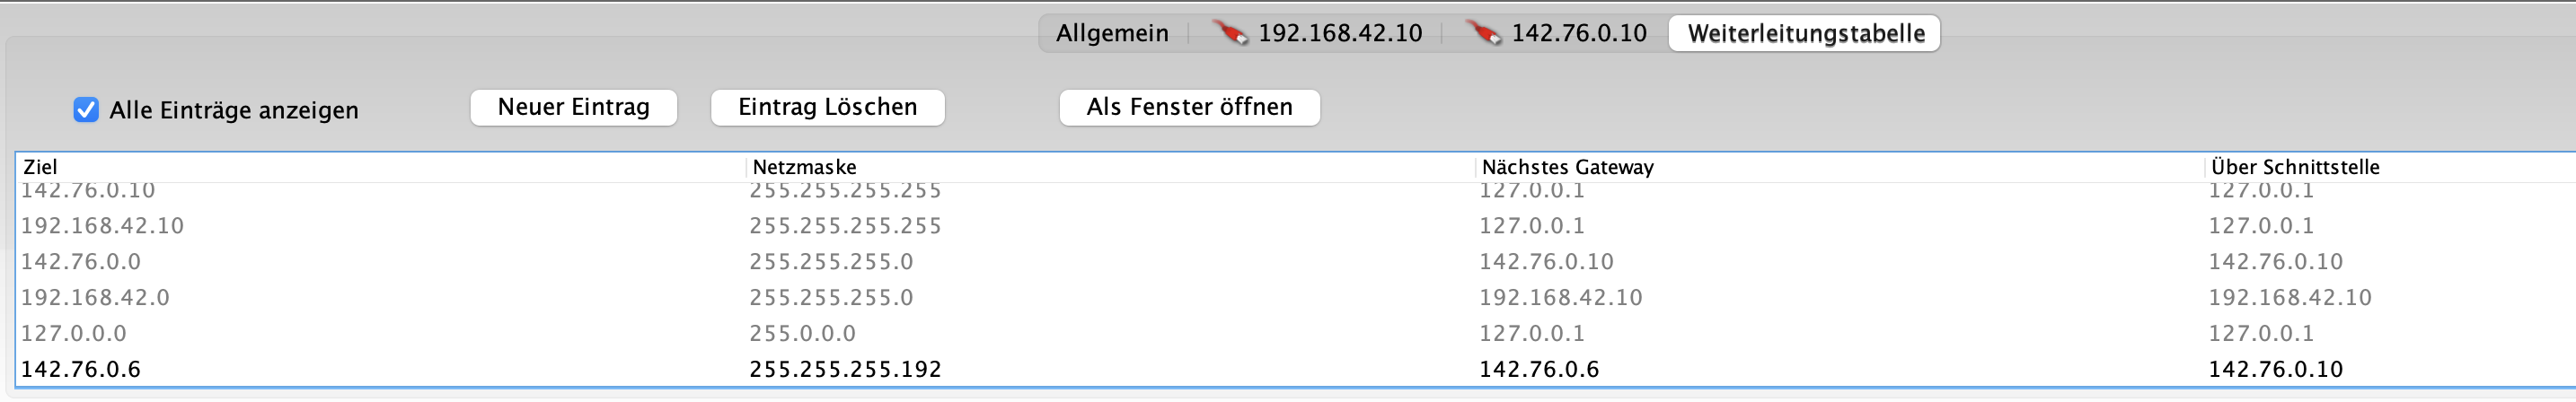
\includegraphics[scale=0.4]{3.4.png}
	\caption{Konfiguration des Vermittlunsgrechners}
	\end{figure}
	\subsection{Webbrowser}
	\begin{figure}[H]
	\centering
	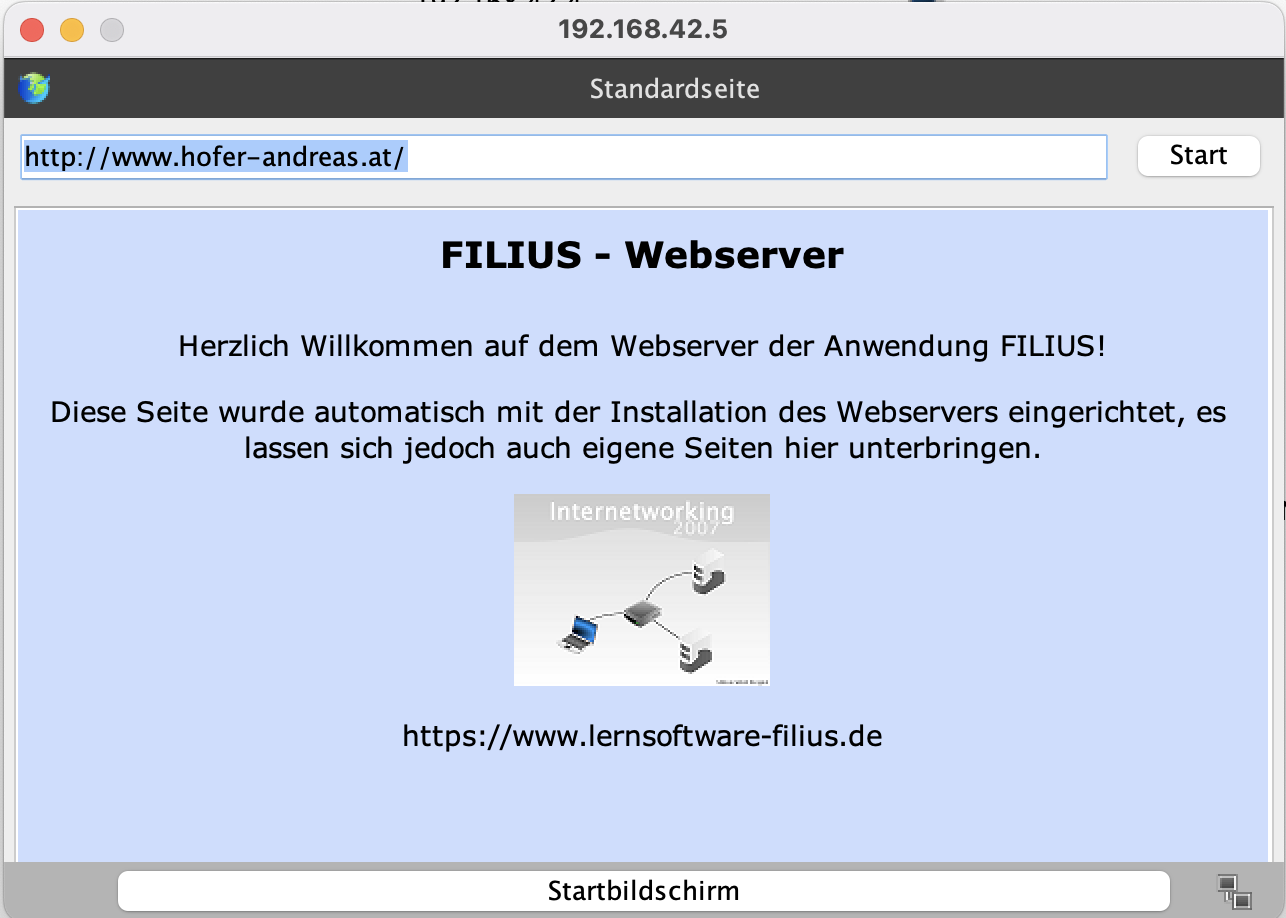
\includegraphics[scale=0.4]{3.5.png}
	\caption{Interface des Webbrowsers}
	\end{figure}
	
	
	
	
	
	
	
	
	
	
\end{document}